\subsection{Tinjauan Studi}

Tinjauan studi bertujuan untuk mengkaji konsep dan pendekatan yang relevan dengan pengembangan aplikasi mobile, implementasi antarmuka pengguna, serta metode pengembangan perangkat lunak yang digunakan dalam penelitian ini. Fokus utama kajian meliputi pemanfaatan framework Flutter dalam pengembangan aplikasi lintas platform, penggunaan Figma sebagai alat perancangan antarmuka, serta penerapan metode Prototype sebagai pendekatan iteratif dalam pengembangan aplikasi.

Pengembangan aplikasi mobile lintas platform menjadi tren karena efisiensi biaya dan waktu pengembangan. Flutter sebagai framework lintas platform menawarkan performa tinggi serta konsistensi antarmuka di berbagai perangkat. Selain itu, penggunaan alat desain UI seperti Figma mendukung kolaborasi antara desainer dan pengembang, sehingga mempermudah proses penerjemahan desain ke dalam implementasi teknis. Metode Prototype dipilih karena sesuai untuk proyek yang menekankan pada iterasi desain dan penyempurnaan antarmuka berdasarkan umpan balik pengguna atau pemangku kepentingan.

Dengan mengombinasikan Flutter, Figma, dan metode Prototype, pengembangan aplikasi Jatidiri diharapkan dapat menghasilkan antarmuka aplikasi yang responsif, konsisten, dan sesuai dengan kebutuhan pengguna.


\subsection{Penelitian Terkait}

Penelitian terkait bertujuan untuk membandingkan penelitian ini dengan penelitian sebelumnya yang relevan.

Kumar \& Sharma (2020) mengembangkan aplikasi mobile lintas platform menggunakan Flutter dan menyimpulkan bahwa Flutter mampu meningkatkan efisiensi pengembangan serta konsistensi tampilan aplikasi.

Hussain et al. (2021) melakukan evaluasi usability pada aplikasi Flutter dan menemukan bahwa kualitas antarmuka pengguna sangat mempengaruhi tingkat kepuasan pengguna.

Santos et al. (2020) melakukan tinjauan sistematis terhadap penggunaan metode Prototype dalam pengembangan perangkat lunak dan menyatakan bahwa metode ini efektif untuk proyek dengan kebutuhan yang berkembang secara iteratif.

Assila et al. (2020) menekankan pentingnya evaluasi usability pada tahap prototyping untuk mengurangi risiko kesalahan desain dan meningkatkan kualitas interaksi pengguna.

Li et al. (2022) membahas penggunaan Figma dalam pengembangan perangkat lunak dan menyatakan bahwa Figma meningkatkan kolaborasi dan mempercepat proses implementasi desain.

Berdasarkan penelitian-penelitian tersebut, dapat disimpulkan bahwa penelitian ini memiliki kebaruan dalam mengombinasikan implementasi UI dari Figma ke Flutter menggunakan metode Prototype dalam konteks aplikasi tes psikologi berbasis mobile.


\subsection{Tinjauan Pustaka}

\subsubsection{Aplikasi Mobile}

Aplikasi mobile adalah perangkat lunak yang dirancang untuk dijalankan pada perangkat bergerak seperti smartphone dan tablet, yang memungkinkan pengguna mengakses berbagai layanan kapan saja dan di mana saja melalui koneksi jaringan atau secara lokal. Aplikasi mobile berperan penting dalam mendukung mobilitas pengguna serta menyediakan interaksi yang cepat dan intuitif melalui antarmuka sentuh dan sensor perangkat (Zhou et al., 2019). Perkembangan aplikasi mobile telah mengubah berbagai sektor, termasuk pendidikan, kesehatan, dan layanan psikologis, dengan menyediakan platform digital yang lebih fleksibel dibandingkan sistem berbasis desktop atau kertas.

Dalam konteks pengembangan perangkat lunak, aplikasi mobile menuntut perhatian khusus terhadap performa, responsivitas, serta pengalaman pengguna karena keterbatasan sumber daya perangkat dan variasi ukuran layar. Oleh karena itu, pengembangan aplikasi mobile tidak hanya berfokus pada fungsionalitas, tetapi juga pada desain antarmuka yang ramah pengguna dan efisien (Rahman et al., 2021). Hal ini menjadikan pemilihan framework dan metode pengembangan yang tepat sebagai faktor penting dalam keberhasilan aplikasi mobile.


\subsubsection{Flutter}

Flutter adalah framework pengembangan aplikasi lintas platform yang dikembangkan oleh Google untuk membangun aplikasi mobile dengan satu basis kode yang dapat dijalankan pada berbagai platform. Flutter menggunakan mesin rendering sendiri dan pendekatan deklaratif dalam membangun antarmuka pengguna, sehingga memungkinkan pengembang menciptakan UI yang konsisten dan responsif (Kumar \& Sharma, 2020). Keunggulan Flutter terletak pada kemampuannya menghasilkan performa yang mendekati native serta menyediakan pustaka widget yang kaya dan fleksibel.

Selain itu, Flutter menyediakan fitur hot reload yang memungkinkan pengembang melihat perubahan kode secara langsung tanpa harus memulai ulang aplikasi, sehingga meningkatkan produktivitas dan mempercepat proses iterasi desain (Hussain et al., 2021). Oleh karena itu, Flutter menjadi pilihan populer dalam pengembangan aplikasi modern yang membutuhkan efisiensi pengembangan, performa tinggi, dan kualitas antarmuka yang baik.


\subsubsection{Dart}

Dart adalah bahasa pemrograman yang dikembangkan oleh Google dan digunakan sebagai bahasa utama dalam framework Flutter. Dart mendukung paradigma pemrograman berorientasi objek dan asinkron, sehingga memungkinkan pengembangan aplikasi yang terstruktur, modular, dan responsif (Barrera \& Hummel, 2021). Dukungan terhadap pemrograman asinkron melalui mekanisme seperti Future dan Stream memungkinkan aplikasi menangani proses latar belakang tanpa mengganggu interaksi pengguna.

Selain itu, Dart memiliki sistem tipe statis dengan fitur null safety yang membantu mengurangi kesalahan runtime dan meningkatkan keandalan kode aplikasi. Hal ini menjadikan Dart cocok untuk pengembangan aplikasi skala menengah hingga besar yang memerlukan maintainability tinggi (Google, 2023).


\subsubsection{Figma}

Figma adalah alat perancangan antarmuka berbasis cloud yang digunakan untuk merancang, memprototipekan, dan mengelola desain UI/UX secara kolaboratif. Figma memungkinkan banyak pengguna bekerja secara bersamaan pada satu dokumen desain, sehingga meningkatkan efisiensi kolaborasi antara desainer dan pengembang (Brown \& Nelson, 2020). Fitur seperti components, styles, dan interactive prototypes membantu menciptakan desain yang konsisten dan mudah disesuaikan selama proses iterasi.

Integrasi Figma dengan proses pengembangan perangkat lunak memungkinkan transisi yang lebih mulus dari desain visual ke implementasi teknis, sehingga mengurangi kesenjangan antara desain dan pengembangan (Li et al., 2022). Oleh karena itu, Figma banyak digunakan dalam pengembangan aplikasi modern yang menekankan kolaborasi tim dan iterasi desain cepat.


\subsubsection{Metode Prototype}

Metode Prototype adalah metode pengembangan perangkat lunak yang menekankan pembuatan purwarupa awal sistem yang kemudian dievaluasi dan disempurnakan secara berulang berdasarkan umpan balik pengguna atau pemangku kepentingan. Pendekatan ini memungkinkan klarifikasi kebutuhan sistem secara bertahap serta mengurangi risiko kesalahan desain yang mahal pada tahap akhir pengembangan (Santos et al., 2020).

Metode Prototype sangat sesuai untuk pengembangan aplikasi yang berfokus pada antarmuka pengguna karena memungkinkan pengujian dini terhadap tampilan dan interaksi sistem. Evaluasi berulang pada tahap prototyping terbukti dapat meningkatkan usability serta kepuasan pengguna terhadap aplikasi yang dikembangkan (Assila et al., 2020).


\subsubsection{Black Box Testing}

Black box testing adalah metode pengujian perangkat lunak yang berfokus pada pengujian fungsi sistem berdasarkan input dan output tanpa memperhatikan struktur internal kode program. Metode ini digunakan untuk memastikan bahwa sistem memenuhi spesifikasi fungsional yang telah ditetapkan (Patton, 2020).

Black box testing banyak digunakan dalam pengujian aplikasi mobile karena memungkinkan pengujian dilakukan dari perspektif pengguna akhir, sehingga membantu mengidentifikasi kesalahan fungsional yang mungkin tidak terlihat dari sisi pengembang (Myers et al., 2021). Dengan demikian, metode ini berperan penting dalam memastikan kualitas dan keandalan aplikasi sebelum digunakan secara luas.


\subsubsection{Visual Studio Code}

Visual Studio Code (VS Code) adalah editor kode sumber ringan yang dikembangkan oleh Microsoft dan широко digunakan dalam pengembangan perangkat lunak modern, termasuk pengembangan aplikasi mobile berbasis Flutter. VS Code mendukung berbagai bahasa pemrograman melalui ekstensi, termasuk Dart dan Flutter, serta menyediakan fitur seperti syntax highlighting, debugging, code completion, dan integrasi dengan sistem kontrol versi Git (Microsoft, 2022). Fitur-fitur ini membantu meningkatkan produktivitas pengembang serta mempermudah proses pengembangan dan pemeliharaan kode.

Selain itu, VS Code mendukung pengembangan lintas platform dan dapat dijalankan pada berbagai sistem operasi, sehingga memudahkan kolaborasi tim dengan lingkungan pengembangan yang konsisten. Kemampuan kustomisasi melalui ekstensi memungkinkan pengembang menyesuaikan editor sesuai dengan kebutuhan proyek, sehingga meningkatkan efisiensi kerja (Sadowski et al., 2018).


\subsubsection{Android}

Android adalah sistem operasi berbasis Linux yang dikembangkan oleh Google untuk perangkat mobile seperti smartphone dan tablet. Android menyediakan platform terbuka bagi pengembang untuk membangun dan mendistribusikan aplikasi kepada pengguna secara luas melalui Google Play Store (Statista, 2023). Sebagai platform mobile yang paling banyak digunakan secara global, Android menjadi target utama dalam pengembangan aplikasi mobile.

Dalam pengembangan aplikasi Jatidiri, Android digunakan sebagai platform utama untuk pengujian dan implementasi aplikasi. Dukungan Android terhadap berbagai ukuran layar, versi sistem operasi, dan perangkat keras menjadikannya platform yang fleksibel tetapi juga menantang dari sisi pengujian kompatibilitas dan performa (Zhou et al., 2019).


\subsubsection{Tes Psikologi}

Tes psikologi adalah instrumen yang digunakan untuk mengukur berbagai aspek psikologis individu, seperti kecerdasan, kepribadian, emosi, motivasi, dan potensi diri. Tes psikologi dirancang berdasarkan prinsip psikometri untuk memastikan validitas dan reliabilitas hasil pengukuran (Flake et al., 2019). Dalam konteks aplikasi Jatidiri, tes psikologi disajikan dalam bentuk digital untuk meningkatkan aksesibilitas dan efisiensi penggunaan.

Penyajian tes psikologi secara digital harus memperhatikan aspek etika, validitas pengukuran, serta interpretasi hasil agar tidak menimbulkan kesalahpahaman bagi pengguna (Coyne et al., 2020). Oleh karena itu, meskipun penelitian ini berfokus pada implementasi teknis aplikasi, pemahaman terhadap konsep dasar tes psikologi tetap menjadi landasan penting dalam pengembangan sistem.


\subsection{RoadMap}

Roadmap pengembangan aplikasi Jatidiri disusun untuk menggambarkan tahapan pelaksanaan proyek secara berkelanjutan mulai dari kegiatan magang Intern 1, Intern 2, hingga penyelesaian pada tahap Tugas Akhir. Roadmap ini terdiri dari tiga fase utama yang saling berkaitan dan berkesinambungan.

\begin{figure}[htbp]
    \centering
    % Roadmap
    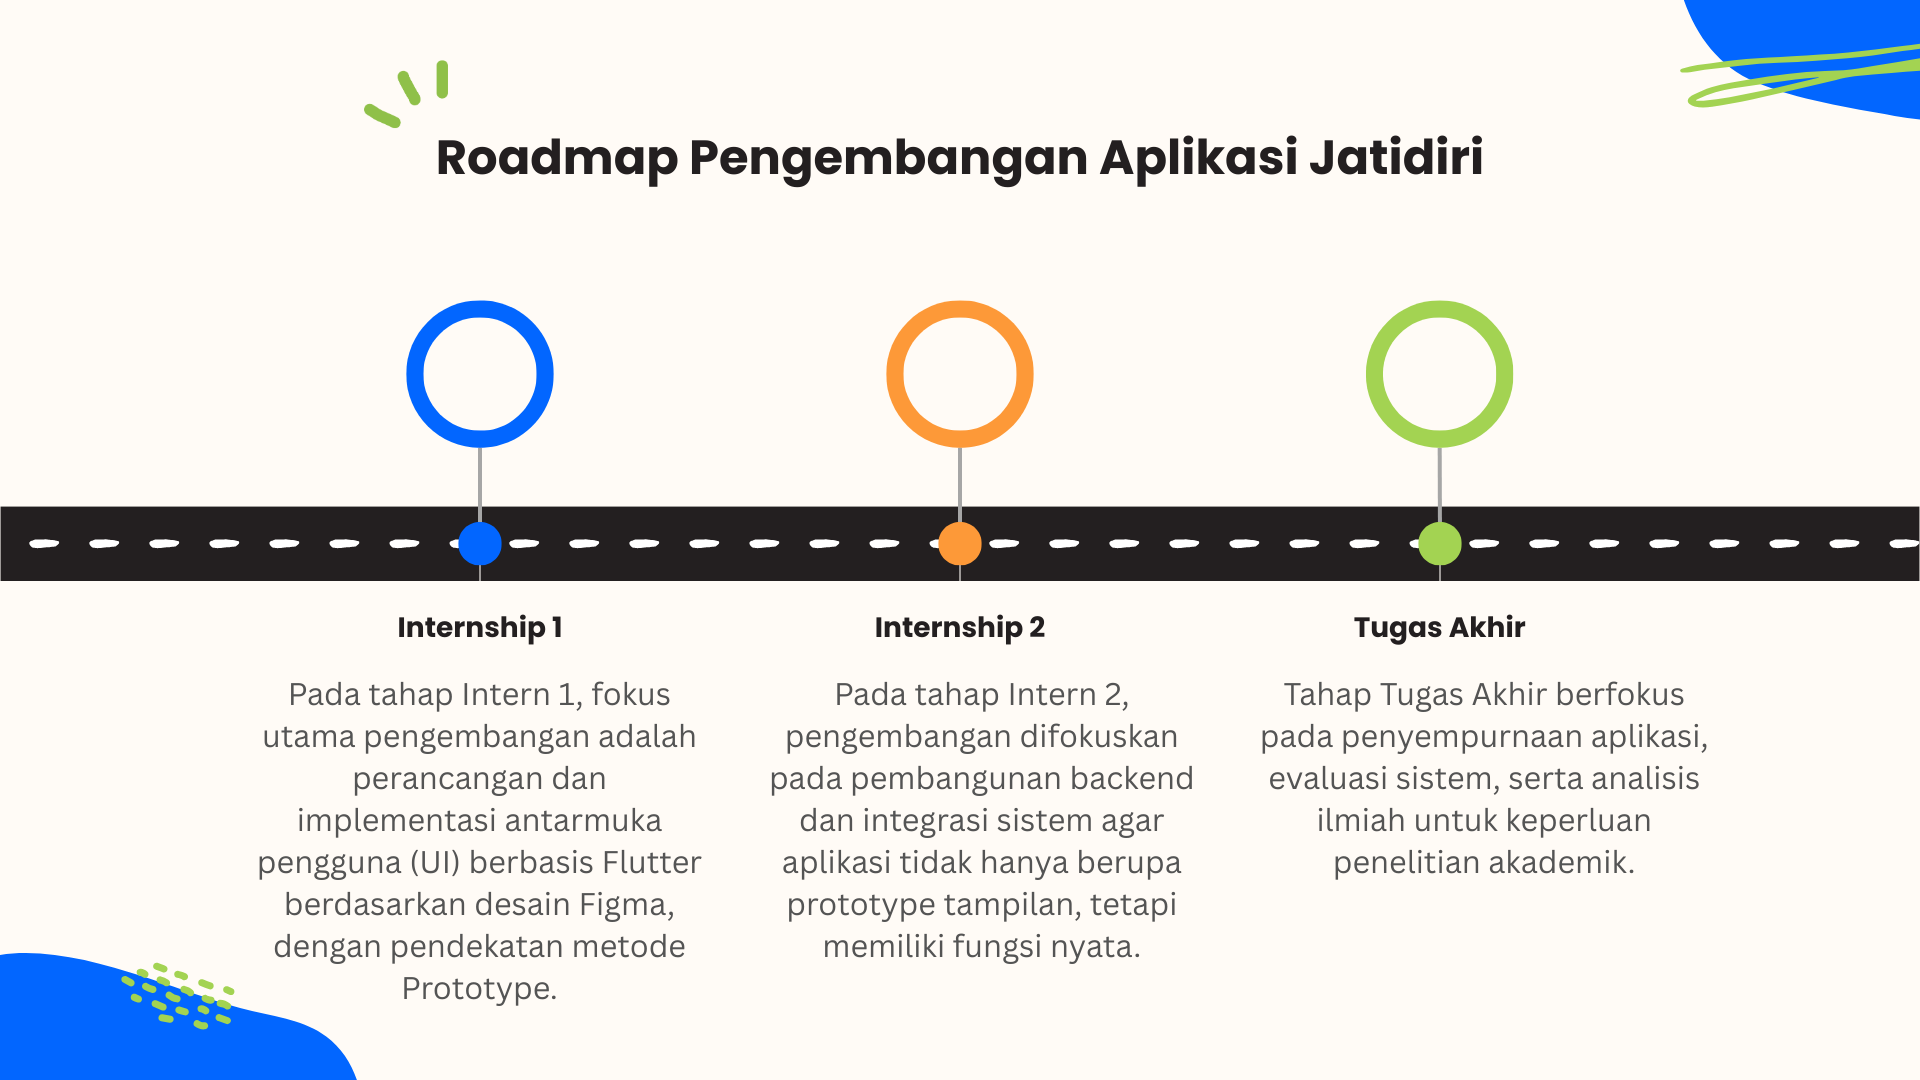
\includegraphics[width=0.6\textwidth]{figures/roadmap.png}
    \caption{Roadmap}
    \label{fig:Roadmap}
\end{figure}